\documentclass{article}
\usepackage{savetrees}
\usepackage{amsmath}
\usepackage{graphicx}
\usepackage{subcaption}
\usepackage{geometry}

\begin{document}
\title{Solution to Assignment 1}
\author{Shoeb Mohammed and Zhuo Chen}
\maketitle

\section{Locally weighted linear regression}

\begin{equation}
  \label{eq:1.1}
  J(\theta) = \frac{1}{2}\sum_{i=1}^m w^{(i)}(\theta^Tx^{(i)}-y^{(i)})^2
\end{equation}

\subsection{}

Matrix $X$ and vectors $\theta$ , $y$ are
\begin{equation}
  \label{eq:1.2}
  X =
  \begin{bmatrix}
    {x^{(i)}}^T \\
    \vdots \\
    {x^{(m)}}^T
  \end{bmatrix}
  ,
  \theta =
  \begin{bmatrix}
    \theta_1 \\
    \vdots \\
    \theta_d
  \end{bmatrix}
  ,
  y =
  \begin{bmatrix}
    y^{(i)} \\
    \vdots \\
    y^{(m)}
  \end{bmatrix}
\end{equation}

Let $W$ be the $m \times m$ diagnoal matrix
\begin{equation}
  \label{eq:1.3}
  W = \frac{1}{2}diag(w^{(1)},\cdots,w^{(m)})
\end{equation}

Using $(\ref{eq:1.2})$ and $(\ref{eq:1.3})$, equation~$(\ref{eq:1.1})$ can be written as
\begin{equation}
  \label{eq:1.4}
  J(\theta) = (X\theta - y)^T W (X\theta - y)
\end{equation}

\subsection{}
The normal equations for un-weighted linear regression are
\begin{equation}
  \label{eq:1.5}
  X^T X \theta = X^T y
\end{equation}
Equation~\ref{eq:1.4} can be re-written as below. Note that 
weights are greater than zero (negative weights don't make sense).
\begin{equation}
  \label{eq:1.6}
  \begin{split}
    J(\theta) &= (X\theta - y)^T \sqrt{W}\sqrt{W} (X\theta - y)     \\
    &= (\sqrt{W}X\theta - \sqrt{W}y)^T (\sqrt{W}X\theta - \sqrt{W}y) \\
    &= (X'\theta - y')^T(X'\theta - y') \text{ where } X' = \sqrt{W}X \text{ and } y' = \sqrt{W}y
  \end{split}
\end{equation}
Now, equation~\ref{eq:1.6} is similar to unweighted $J(\theta)$. Thus, using equation~\ref{eq:1.5}, $\theta$ in closed form is
\begin{equation}
  \label{eq:1.7}
  \begin{split}
    \theta &= \left[(\sqrt{W}X)^T(\sqrt{W}X)\right]^{-1} \left(\sqrt{W}X\right)^T \sqrt{W}y \\
  \end{split}
\end{equation}

\subsection{}
Locally weighted linear regression is a non-parametric model.
To estimate $y$, given $x$

\begin{itemize}
\item first calculate the weights $w^{(i)}$. This gives the matrix $W$ as defined in equation~\ref{eq:1.3}
\item Start with random guess for $\theta$
  \item In the i\textsuperscript{th} iteration of the algorithm, the $\theta$ is updated using the relation
    \begin{equation}
      \label{eq:1.8}
      \theta(i) \leftarrow \theta(i-1) - \alpha \left(\sqrt{W}X\right)^T \left(\sqrt{W}X\theta(i-1) - \sqrt{W}y\right)
    \end{equation}
\item The above step is repeated until $\theta$ converges
\end{itemize}

\section{Properties of the linear regression estimator}
\subsection{}
Vectors $y, \theta , \epsilon$ and matrix $X$ are related as
\begin{equation}
  \label{eq:1.9}
  y = X \theta + \epsilon
\end{equation}
$\epsilon$ is i.i.d $N(0,\sigma^{2})$.

Thus, for the optimal value $\theta^{*}$ and fixed $X$
\begin{equation}
  \label{eq:1.10}
  \begin{split}
    E[y] &= E[X\theta^{*}] + E[\epsilon]\\
    &= E[X\theta^{*}] + 0\\
    &= X\theta^{*}
  \end{split}
\end{equation}

Given the normal equations
\begin{equation}
  \label{eq:1.11}
  \begin{split}
  \theta &= (X^T X)^{-1}X^T y \\
  \implies E[\theta] &= (X^T X)^{-1}X^T E[y] \\
  &= (X^T X)^{-1}X^T X\theta^{*} \\
  &= \theta^{*}    
  \end{split}
\end{equation}

\subsection{}
\begin{equation}
  \label{eq:1.12}
  \begin{split}
    Var(\theta) &= E\left[(\theta - E(\theta))(\theta - E(\theta))^T\right] \\
    &= E\left[(\theta - \theta^*)(\theta - \theta^*)^T\right] \\
    &= E[\theta \theta^T] - \theta^*{\theta^*}^T
  \end{split}
\end{equation}

Use the normal equations (linear regression estimator) to get
\begin{equation}
  \label{eq:1.13}
  \begin{split}
    E[\theta\theta^T] &= E\left[ (X^TX)^{-1} X^T yy^T \left( (X^TX)^{-1} \right)^T \right] \\    
    &= (X^TX)^{-1} X^T E[yy^T] \left( (X^TX)^{-1} \right)^T
  \end{split}
\end{equation}
Use equation~\ref{eq:1.9} to get 
\begin{equation}
  \label{eq:1.14}
  \begin{split}
    E[yy^T] &= E[(X\theta + \epsilon) (X\theta + \epsilon) \\
    &= E[X\theta^* {\theta^*}^T X^T + X\theta^*\epsilon^T + \epsilon {\theta^*}^T X^T + \epsilon\epsilon^T] \\
    &= X\theta^* {\theta^*}^T X^T + E[\epsilon\epsilon^T] \\
    &= X\theta^* {\theta^*}^T X^T + diag(\sigma^2) \\
    &= X\theta^* {\theta^*}^T X^T + \sigma^2 I
  \end{split}
\end{equation}

Equations~\ref{eq:1.13} and~\ref{eq:1.14} imply
\begin{equation}
  \label{eq:1.15}
  \begin{split}
    E[\theta\theta^T] &= (X^TX)^{-1} X^T \left[X\theta^* {\theta^*}^T X^T + \sigma^2 I \right] X\left( (X^TX)^{-1} \right)^T \\
    &= \left[\theta^* {\theta^*}^T X^T + (X^TX)^{-1} X^T \sigma^2 I \right] X \left( (X^TX)^{-1} \right)^T \\ 
    &= \theta^* {\theta^*}^T + (X^TX)^{-1} X^T \sigma^2 I X \left( (X^TX)^{-1} \right)^T \\
    &= \theta^* {\theta^*}^T + \sigma^2 (X^TX)^{-1} X^T X \left( (X^TX)^{-1} \right)^T \\
    &= \theta^* {\theta^*}^T + \sigma^2 (X^TX)^{-1}
  \end{split}
\end{equation}
Equations~\ref{eq:1.12} and~\ref{eq:1.15} imply
\begin{equation}
  \label{eq:1.16}
  Var(\theta) = \sigma^2 (X^TX)^{-1}
\end{equation}
\section{Problem 3: Part 1: Implementing  linear regression}

\begin{table}[h]
	\caption{Files modified and plots generated for Problem3: Part1} \centering
	\begin{tabular}{l|l|l|l|}
		\hline\hline
		Problem & function implemented & Files edited & Output and Plots\\
		\hline\hline
		3.1.A1  & \verb|LinearReg_SquaredLoss.loss| & \verb|linear_regressor.py| & Fig~\ref{fig:1}  \\
		
		3.1.A2  & \verb|LinearRegressor.train| & \verb|linear_regressor.py| and \verb|ex1.py| & Fig~\ref{fig:2},Fig~\ref{fig:3} and Fig~\ref{fig:4}\\
		
		3.1.A3  & \verb|LinearRegressor.predict| & \verb|linear_regressor.py| and \verb|ex1.py| &  \\
		
		3.1.B1  & \verb|feature_normalize| & \verb|utils.py| & \\
		
		3.1.B2  & \verb|LinearRegressor.train| & \verb|linear_regressor_multi.py| & Fig~\ref{fig:5}\\
		
	  & \verb|LinearReg_SquaredLoss.loss| &  & \\
		%\verb|Error at lambda = 1.0 (problem3.2.A6) is  3.0987791808| \\
		
		3.1.B3  &  & \verb|ex1_multi.py| & \\
		3.1.B4  & \verb|LinearRegressor_Multi.normal_equation| &\verb|linear_regressor_multi.py| and \verb|ex1_multi.py| & \\
		3.1.B5  &  & \verb|ex1_multi.py| & Fig~\ref{fig:66}\\
		\hline
	\end{tabular} \label{table:prob3_part1_summary}
\end{table}
\subsection{Problem 3.1.A}
\begin{itemize}
	\item Implemented the \verb|LinearReg_SquaredLoss.loss| and \verb|LinearRegressor.train| methods in file
	\verb|linear_regressor.py|. 
	\item Add code in 	\verb|ex1.py| to predict median home values at LSTAT = 5\% and 50\%.
	\item $\theta$ predicted: $[34.55363411, -0.95003694]$
	\item Median home values predicted:\\
	LSTAT = 5\%: 298034.494122\\
	LSTAT = 50\%: -129482.128898
	
\end{itemize}
\subsection{Problem 3.1.B}

\begin{itemize}
	\item Implemented the \verb|feature_normalize| method in file
	\verb|utils.py| to normalize the data. 
	\item Implemented the \verb|LinearRegressor.train| and \verb|LinearReg_SquaredLoss.loss| methods in file
	\verb|linear_regressor_multi.py|. 
	\item Add code in 	\verb|ex1_multi.py| to predict median home values at average home.
	\item Add code in 	\verb|ex1_multi.py| to explore convergence of gradient descent.
	\item For average home in Boston suburbs, we predict a median home value of 225328.063241 using gradient descent.
	\item For average home in Boston suburbs, we predict a median home value of 225328.06324113 using normal equation.
	\item When learning rate >=1, the loss function could not convergent. So $alpha$ = 0.3 is a good learning rate and 10 iteration is enough for that.
\end{itemize}

\begin{figure}[h]
	\centering{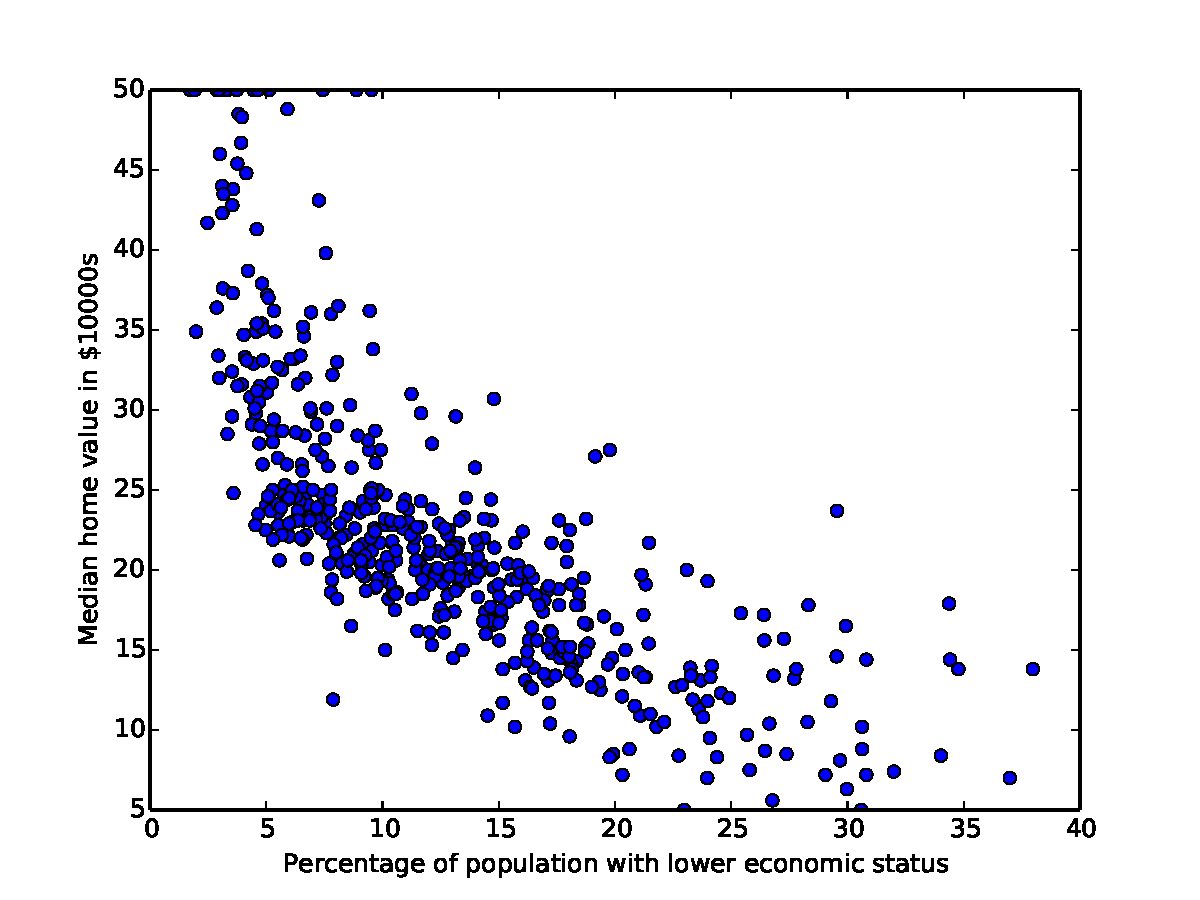
\includegraphics[width=15cm]{part1/fig1.pdf}}
	\caption{The training data for linear regression.}\label{fig:1}
\end{figure}

\begin{figure}[h]
	\centering{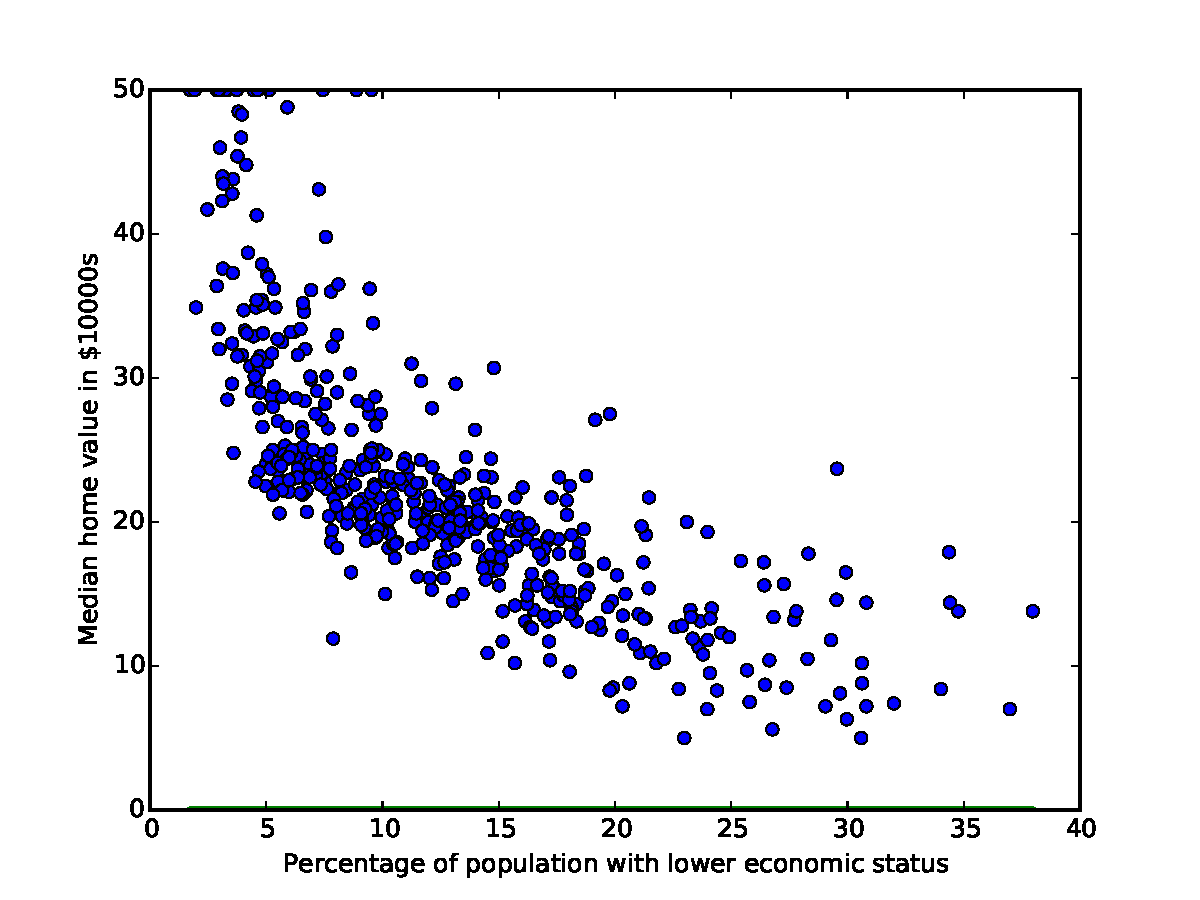
\includegraphics[width=15cm]{part1/fig2.pdf}}
	\caption{Fitting a linear model to the data in Fig~\ref{fig:1}}\label{fig:2}
\end{figure}

\begin{figure}[h]
	\centering{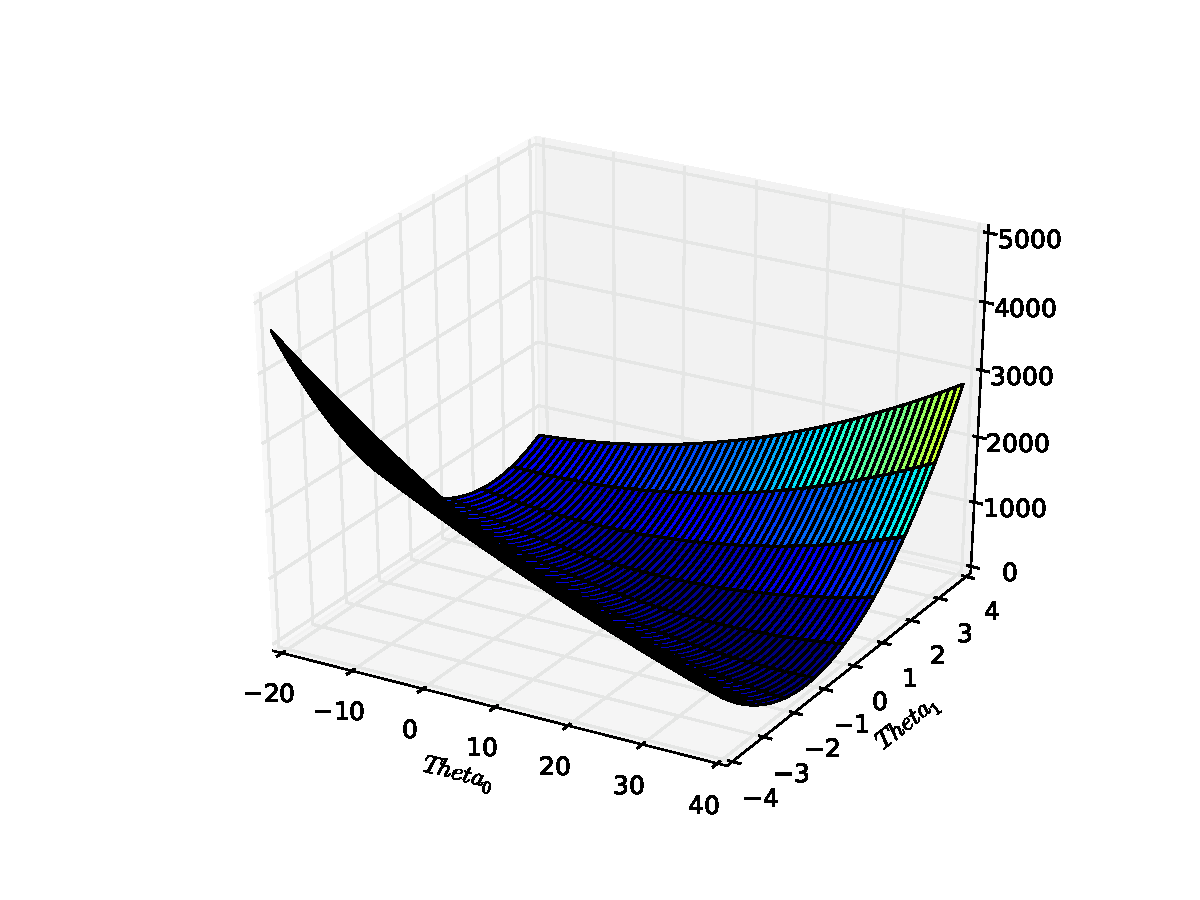
\includegraphics[width=7cm]{part1/fig3a.pdf}}
		\centering{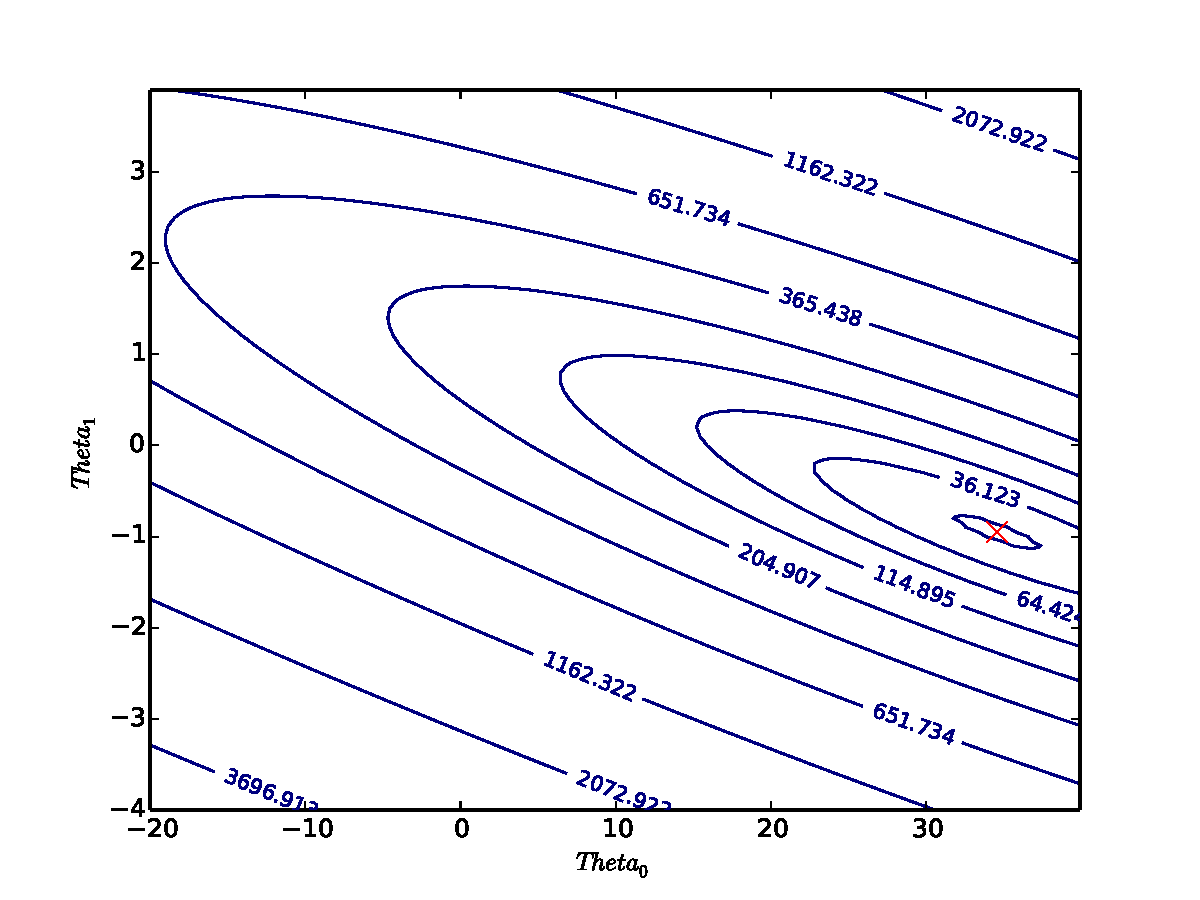
\includegraphics[width=7cm]{part1/fig3b.pdf}}
	\caption{Surface and contour plot of cost function}\label{fig:3}
\end{figure}

\begin{figure}[h]
	\centering{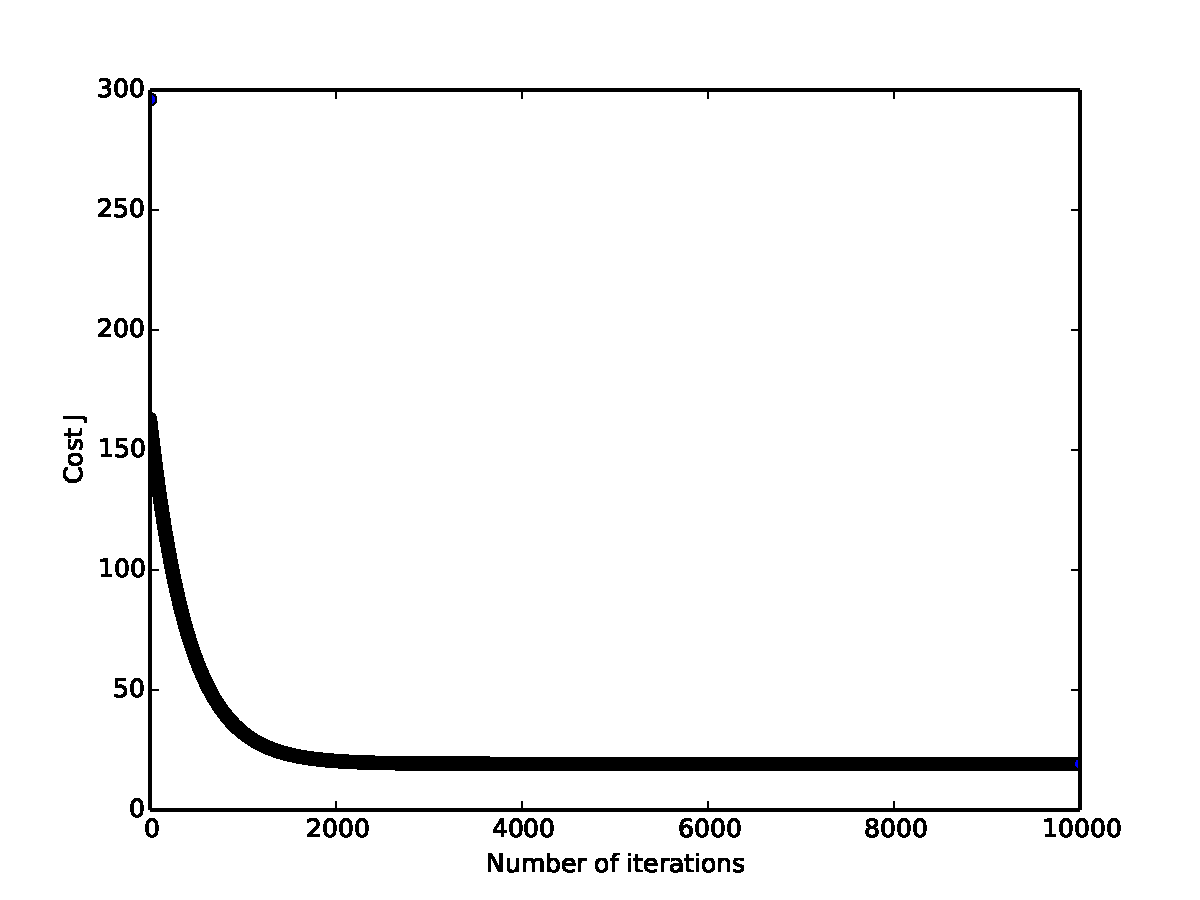
\includegraphics[width=7cm]{part1/fig4.pdf}}

	\caption{Convergence of gradient descent for linear regression with single variables}\label{fig:4}
\end{figure}
\begin{figure}[h]
	\centering{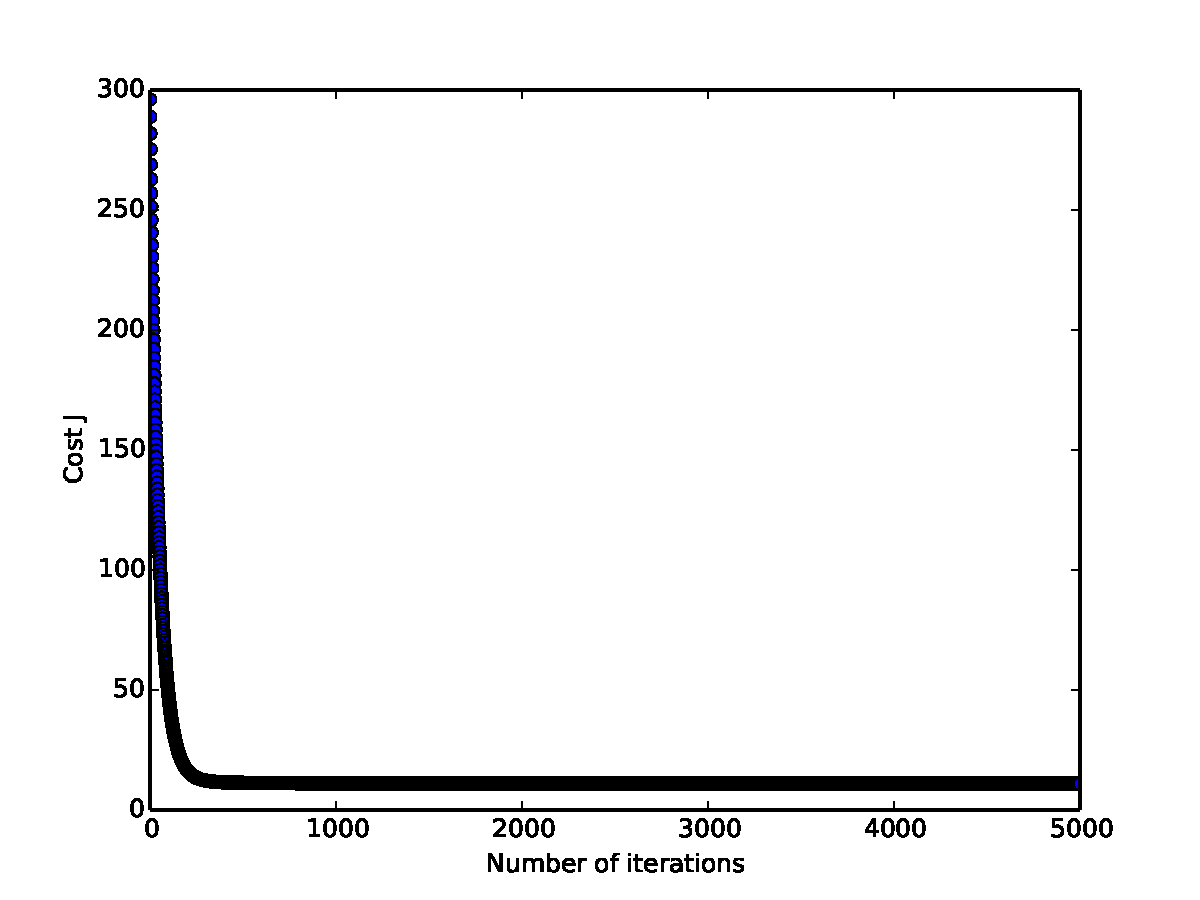
\includegraphics[width=7cm]{part1/fig5.pdf}}
	
	\caption{Convergence of gradient descent for linear regression with multi variables}\label{fig:5}
\end{figure}
\begin{figure}[h]
\centering{\includegraphics[width=7cm]{part1/fig6_1.pdf}}
\centering{\includegraphics[width=7cm]{part1/fig6_2.pdf}}
\centering{\includegraphics[width=7cm]{part1/fig6_3.pdf}}
\centering{\includegraphics[width=7cm]{part1/fig6_4.pdf}}
\centering{\includegraphics[width=7cm]{part1/fig6_5.pdf}}
\centering{\includegraphics[width=7cm]{part1/fig6_6.pdf}}
\caption{Convergence of gradient descent for linear regression with multi variables at different learning rate: $alpha$=0.01,0.03,0.1,0.3,1,3}
\label{fig:66}
\end{figure}

\section{Problem 3: Part 2: Implementing regularized linear regression}

\begin{table}[h]
\caption{Files modified and plots generated for Problem3: Part2} \centering
\begin{tabular}{l|l|l|l|}
\hline\hline
Problem & function implemented & Files edited & Output and Plots\\
\hline\hline
3.2.A1  & \verb|RegularizedLinearReg_SquaredLoss.loss| & \verb|reg_linear_regressor_multi.py| & Fig~\ref{fig:6} and Fig~\ref{fig:7}\\

3.2.A2  & \verb|RegularizedLinearReg_SquaredLoss.grad_loss| & \verb|reg_linear_regressor_multi.py| & Fig~\ref{fig:6} and Fig~\ref{fig:7}\\

3.2.A3  & \verb|learning_curve| and \verb|feature_normalize| & \verb|utils.py| & Fig~\ref{fig:8}, Fig~\ref{fig:9} and Fig~\ref{fig:10} \\

3.2.A4  & - & \verb|ex2.py| added code for $\lambda=1,10,100$ & Fig~\ref{fig:9_10_reg}\\

3.2.A5  & \verb|validation_curve| & \verb|utils.py| & Fig~\ref{fig:12}\\

3.2.A6  & - & \verb|ex2.py| added code for $\lambda=1$ from prob3.2.A5 & \verb|Error=3.0987791808|\\
%\verb|Error at lambda = 1.0 (problem3.2.A6) is  3.0987791808| \\

3.2.A7  & \verb|averaged_learning_curve| & \verb|utils.py| & Fig~\ref{fig:11}\\
\hline
\end{tabular} \label{table:prob3_part2_summary}
\end{table}

\subsection{Problem 3.2.A1 and Problem 3.2.A2:}
\begin{itemize}
\item Implemented the \verb|RegularizedLinearReg_SquaredLoss.loss| and \verb|RegularizedLinearReg_SquaredLoss.grad_loss| methods in file
  \verb|reg_linear_regressor_multi.py| per requirements of the problem. 
\end{itemize}
The updated methods use regularized regression to calculate the loss and gradient. The output from \verb|ex2.py| is shown in Fig~\ref{fig:6} and Fig~\ref{fig:7}.

\begin{figure}[h]
  \centering{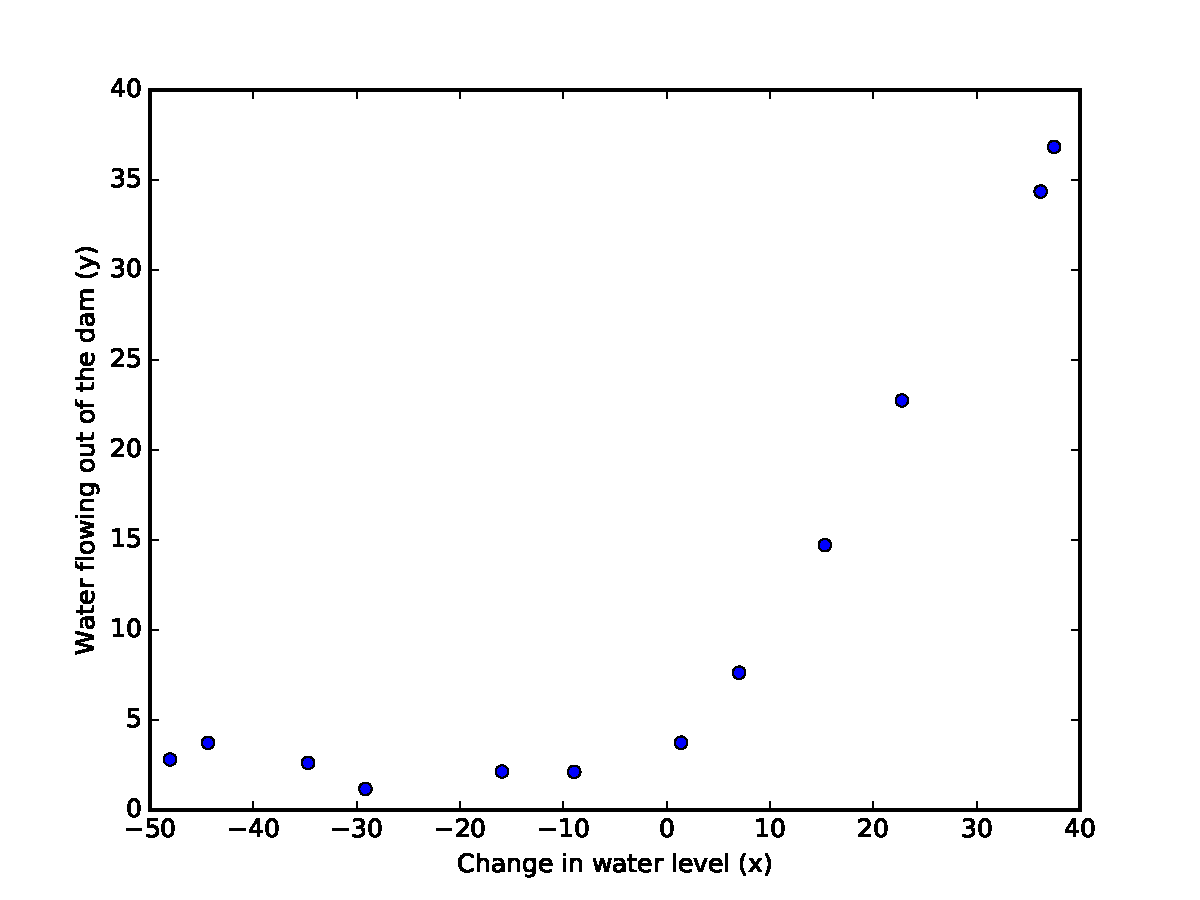
\includegraphics[width=15cm]{part2/fig6.pdf}}
  \caption{The training data for regularized linear regression.}\label{fig:6}
\end{figure}

\begin{figure}[h]
  \centering{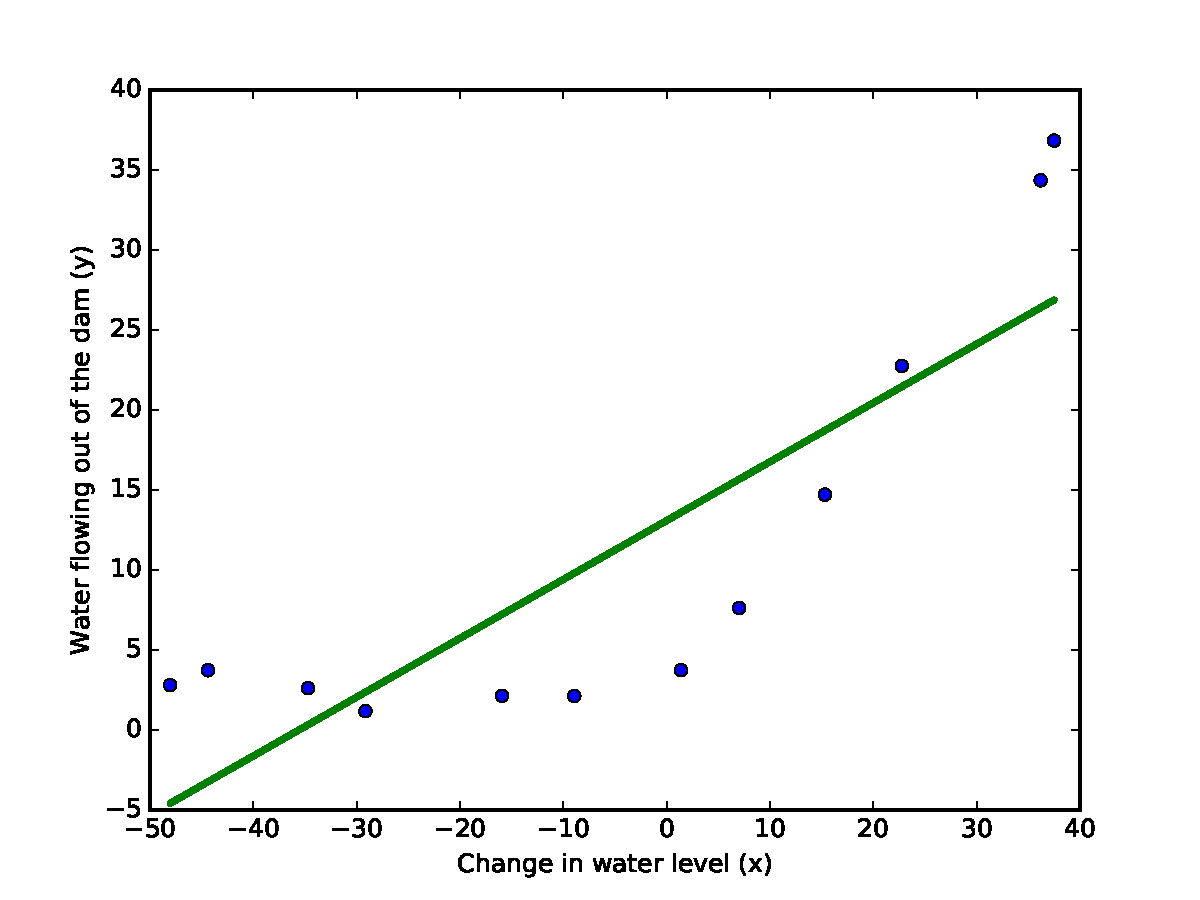
\includegraphics[width=15cm]{part2/fig7.pdf}}
  \caption{The best fit line for the training data.}\label{fig:7}
\end{figure}

\subsection{Problem 3.2.A3}
\begin{itemize}
\item Implemented the \verb|learning_curve| function in file \verb|utils.py| per the requirements of the problem. The output from
  \verb|ex2.py| is shown in Fig~\ref{fig:8}
\item Implemented the \verb|feature_normalize| function in file \verb|utils.py|. The output from \verb|ex2.py| is shown in
  Fig~\ref{fig:9} and Fig~\ref{fig:10}
\end{itemize}

\begin{figure}[h]
  \centering{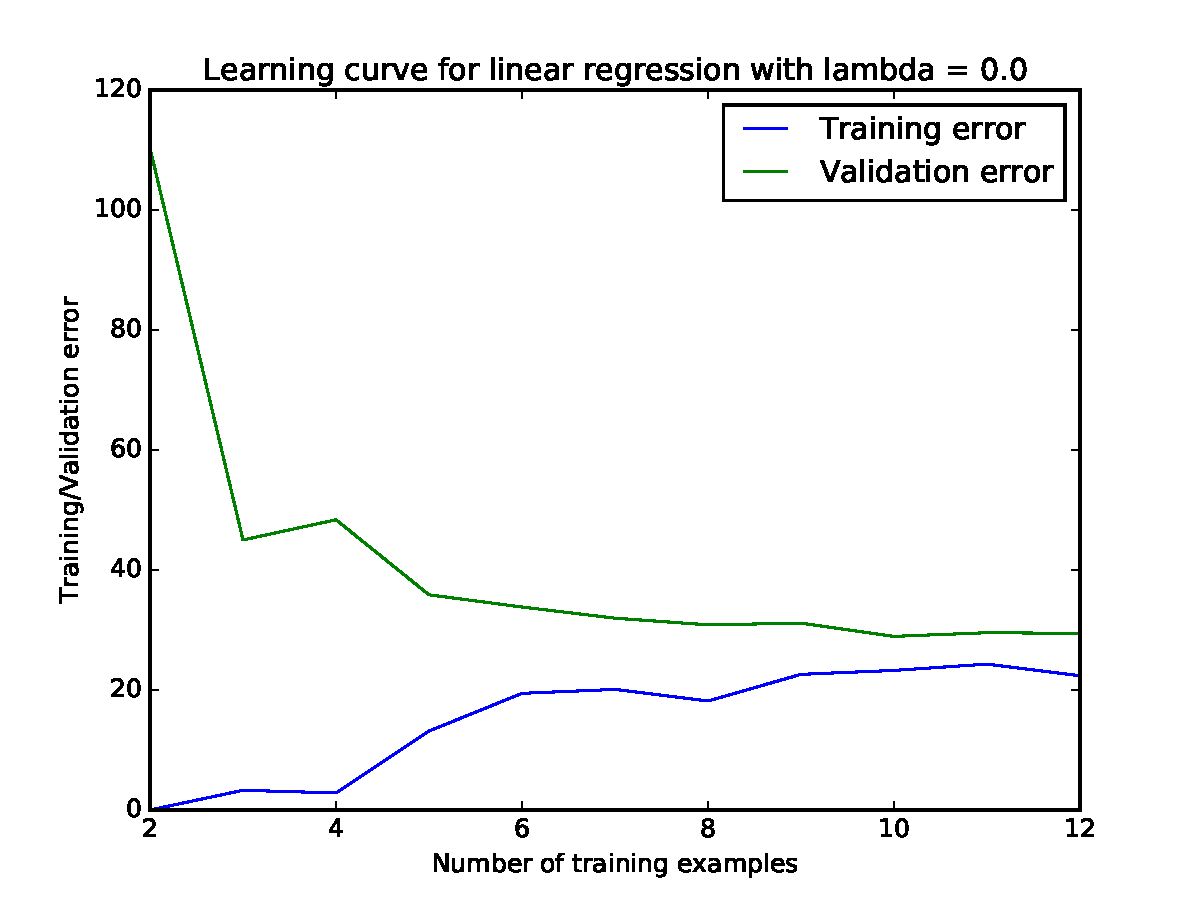
\includegraphics[width=15cm]{part2/fig8.pdf}}
  \caption{Learning curves.}\label{fig:8}
\end{figure}

\begin{figure}[h]
  \centering{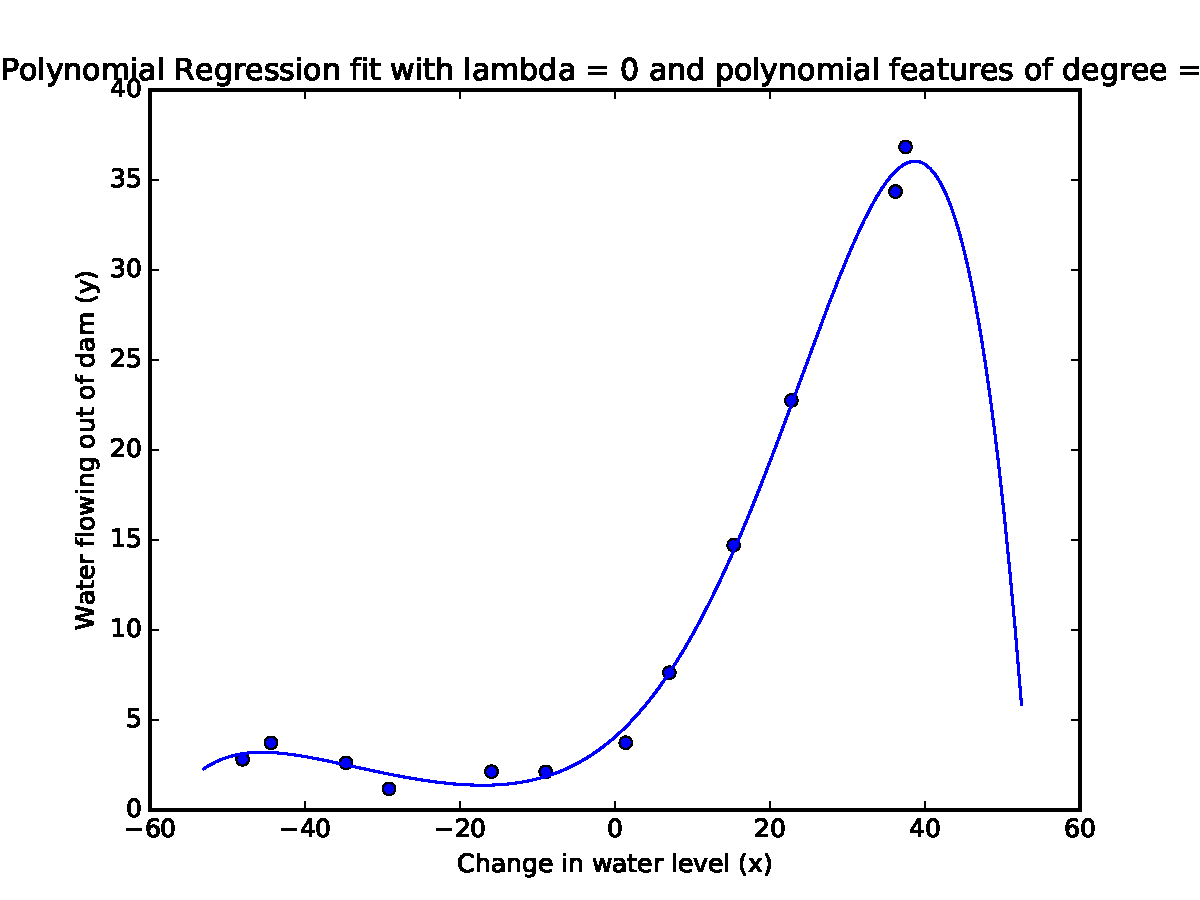
\includegraphics[width=15cm]{part2/fig9.pdf}}
  \caption{Polynomial fit for lambda = 0 with a p=8 order model.}\label{fig:9}
\end{figure}

\begin{figure}
  \centering{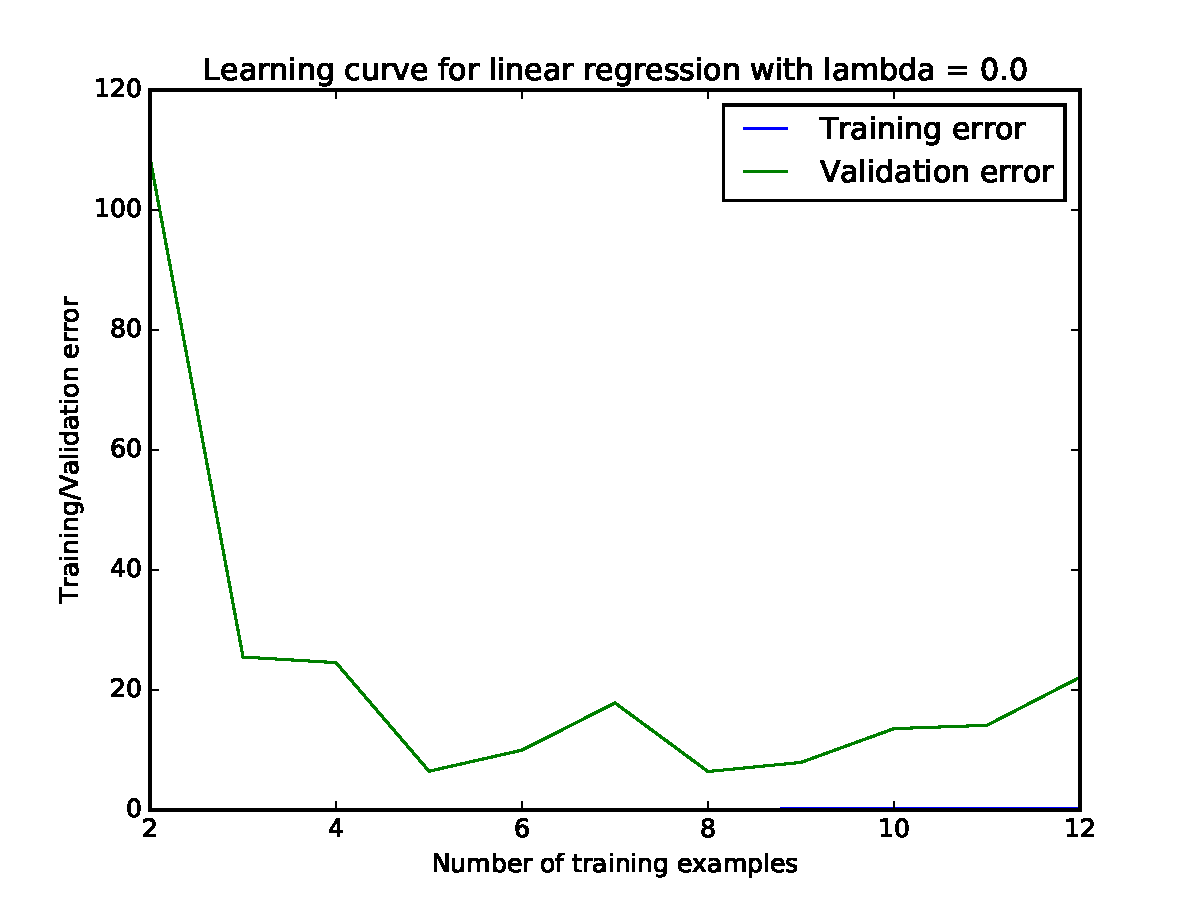
\includegraphics[width=15cm]{part2/fig10.pdf}}
  \caption{Learning curve for lambda = 0.}\label{fig:10}
\end{figure}

\subsection{Problem 3.2.A4}
\begin{itemize}
\item The results for $\lambda = 1.0$ are shown in Fig~\ref{fig:9_reg1} and Fig~\ref{fig:10_reg1}.
\item The results for $\lambda = 10.0$ are shown in Fig~\ref{fig:9_reg10} and Fig~\ref{fig:10_reg10}.
\item The results for $\lambda = 100.0$ are shown in Fig~\ref{fig:9_reg100} and Fig~\ref{fig:10_reg100}.
\end{itemize}

We observe that low value of the regularization parameter $\lambda$ is strongly biased while a large value
for $\lambda$ has high variance.

\newgeometry{left=0.5cm,right=0.5cm,top=0.5cm,bottom=4cm}
\begin{figure}[h]
  \subcaptionbox{Polynomial fit for lambda = 1 with a p=8 order model.\label{fig:9_reg1}}
  [.5\linewidth]{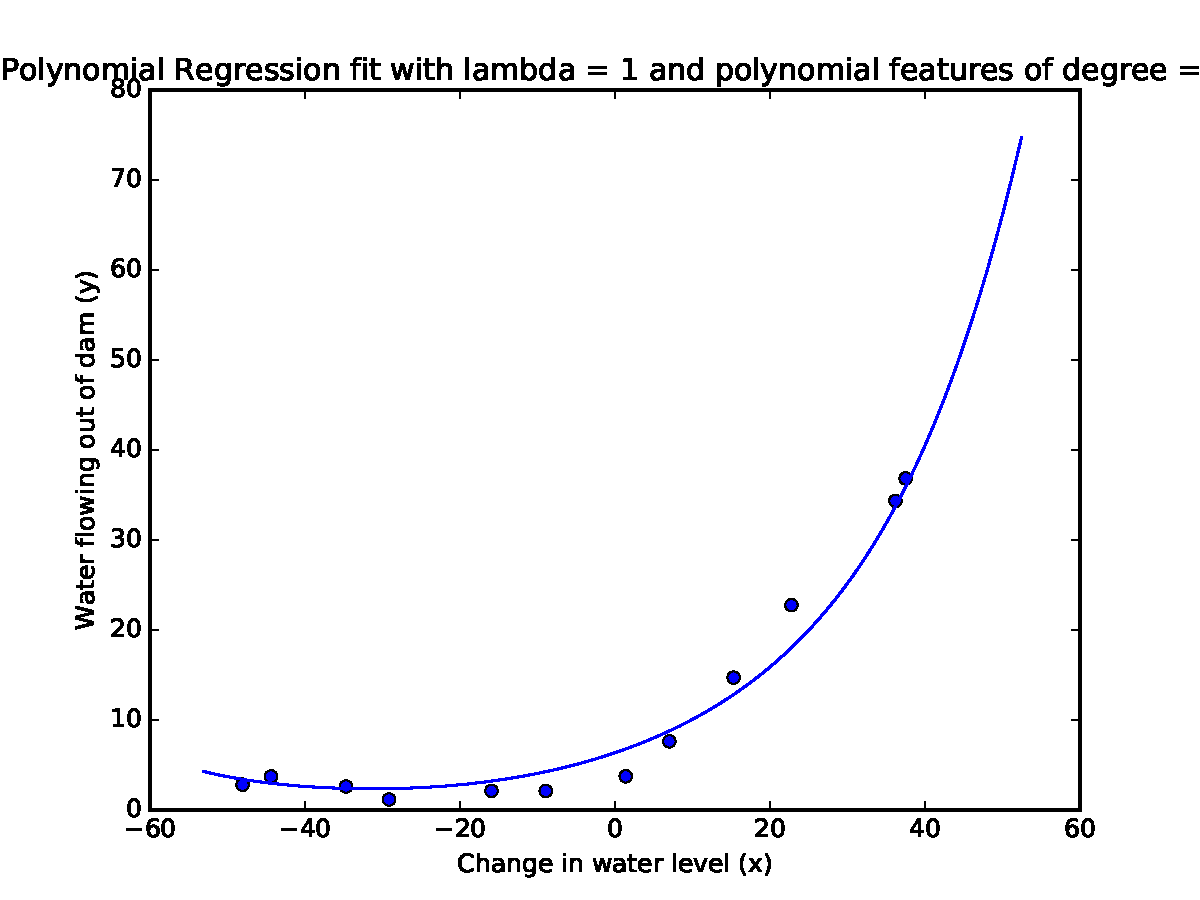
\includegraphics[width=9cm]{part2/fig9_reg1.pdf}}%
  \subcaptionbox{Learning curve for lambda = 1.\label{fig:10_reg1}}
  [.5\linewidth]{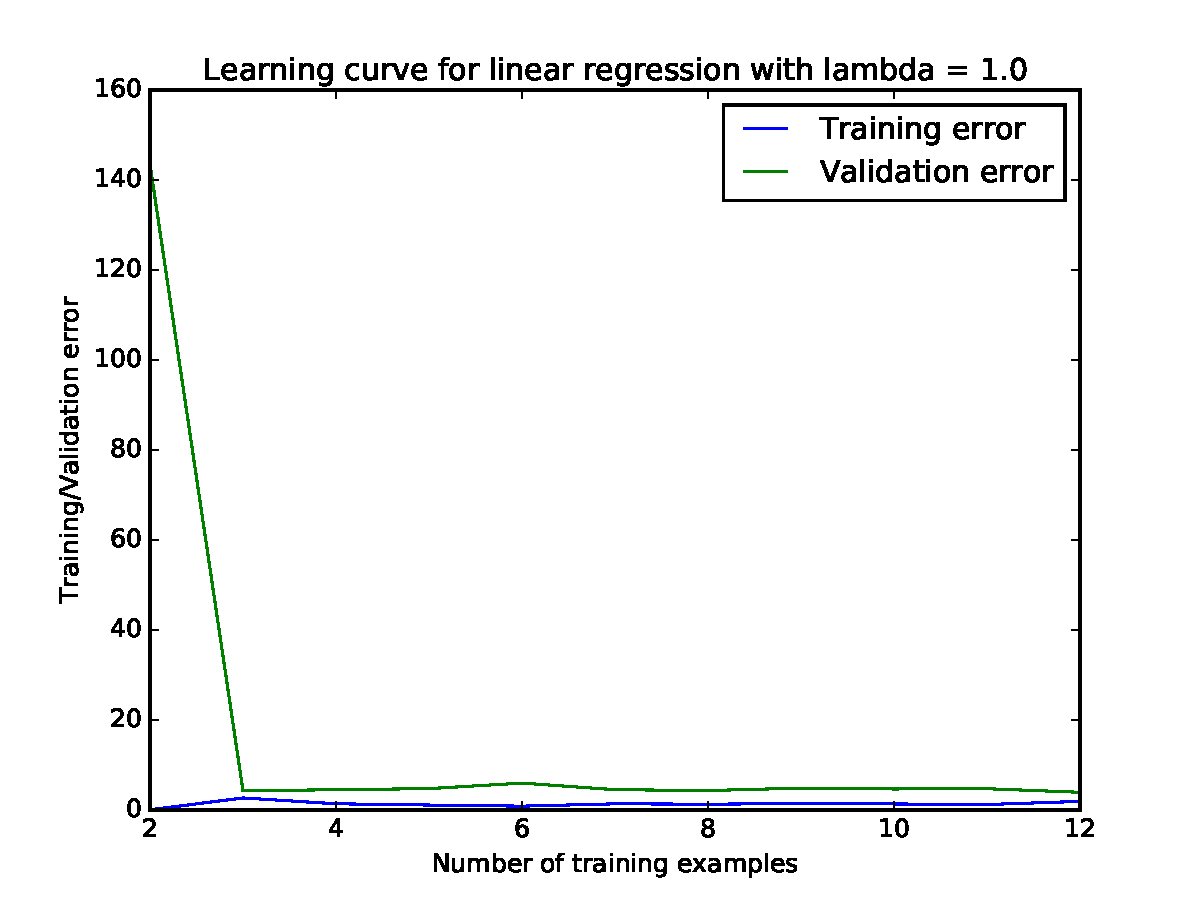
\includegraphics[width=9cm]{part2/fig10_reg1.pdf}}
  
  \subcaptionbox{Polynomial fit for lambda = 10 with a p=8 order model.\label{fig:9_reg10}}
  [.5\linewidth]{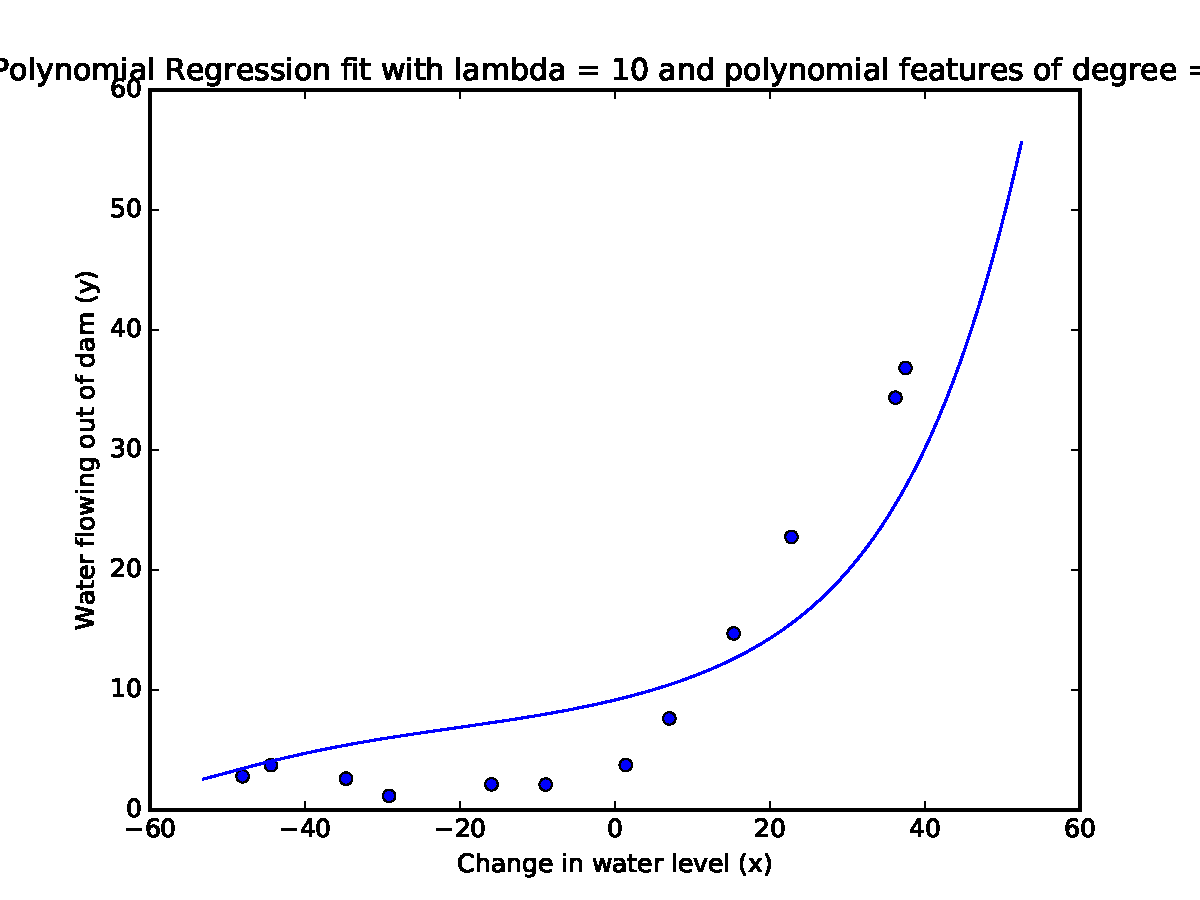
\includegraphics[width=9cm]{part2/fig9_reg10.pdf}}%
  \subcaptionbox{Learning curve for lambda = 10.\label{fig:10_reg10}}
  [.5\linewidth]{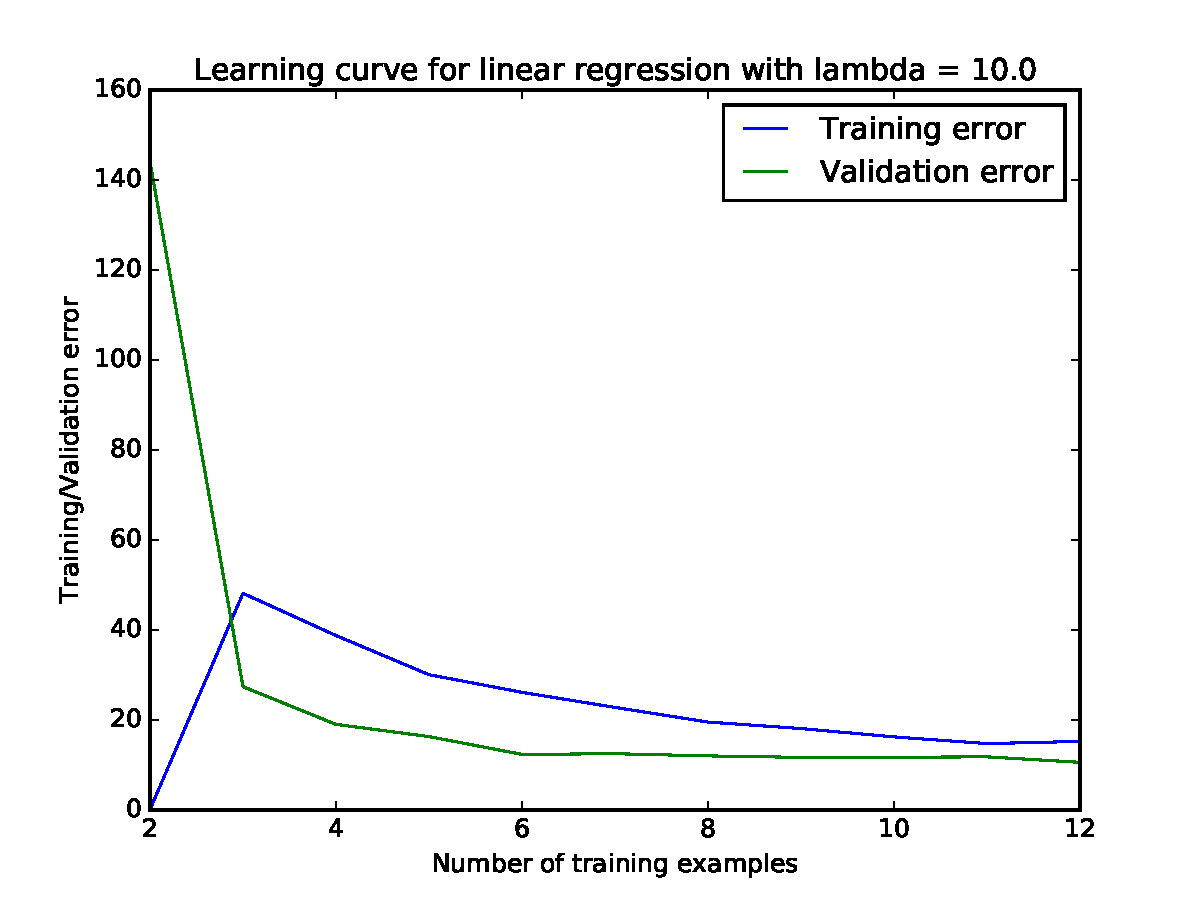
\includegraphics[width=9cm]{part2/fig10_reg10.pdf}}

  \subcaptionbox{Polynomial fit for lambda = 100 with a p=8 order model.\label{fig:9_reg100}}
  [.5\linewidth]{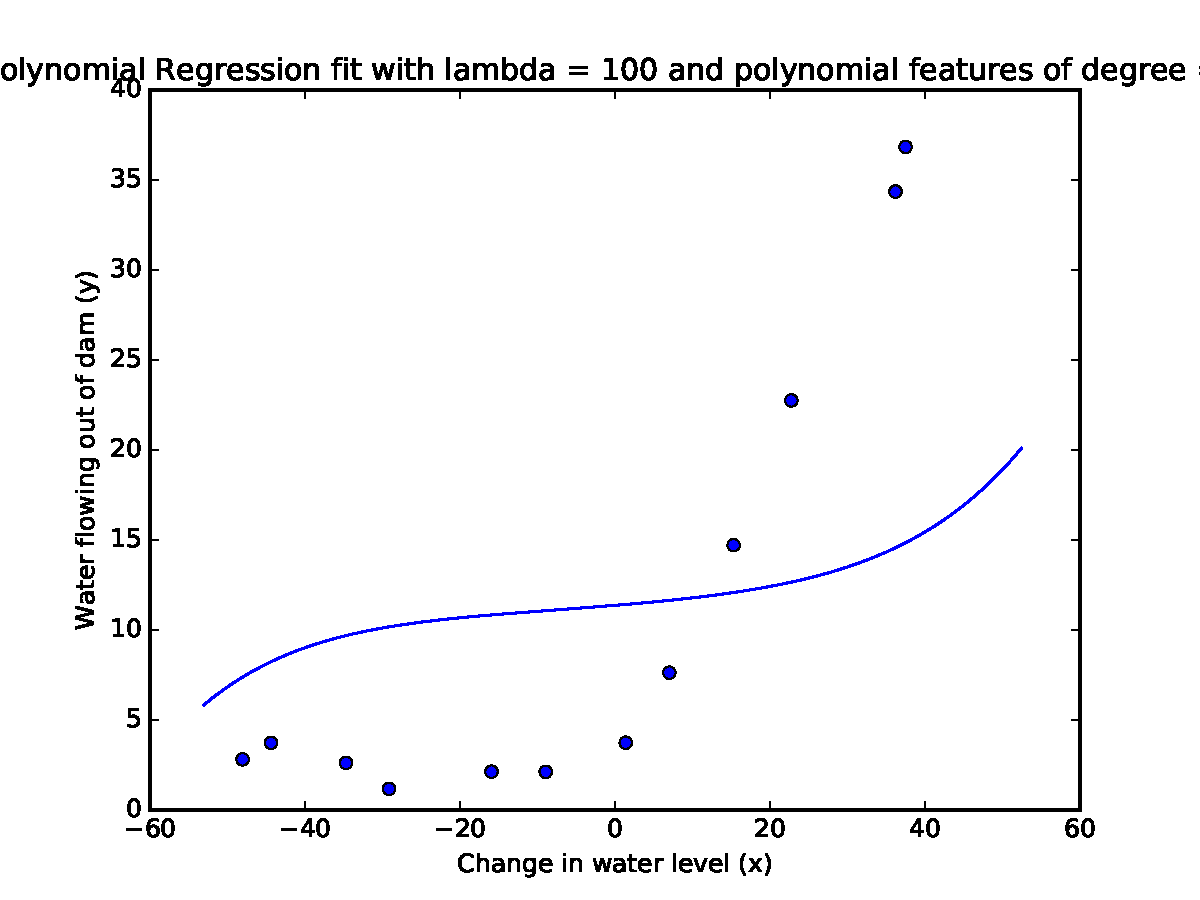
\includegraphics[width=9cm]{part2/fig9_reg100.pdf}}%
  \subcaptionbox{Learning curve for lambda = 100.\label{fig:10_reg100}}
  [.5\linewidth]{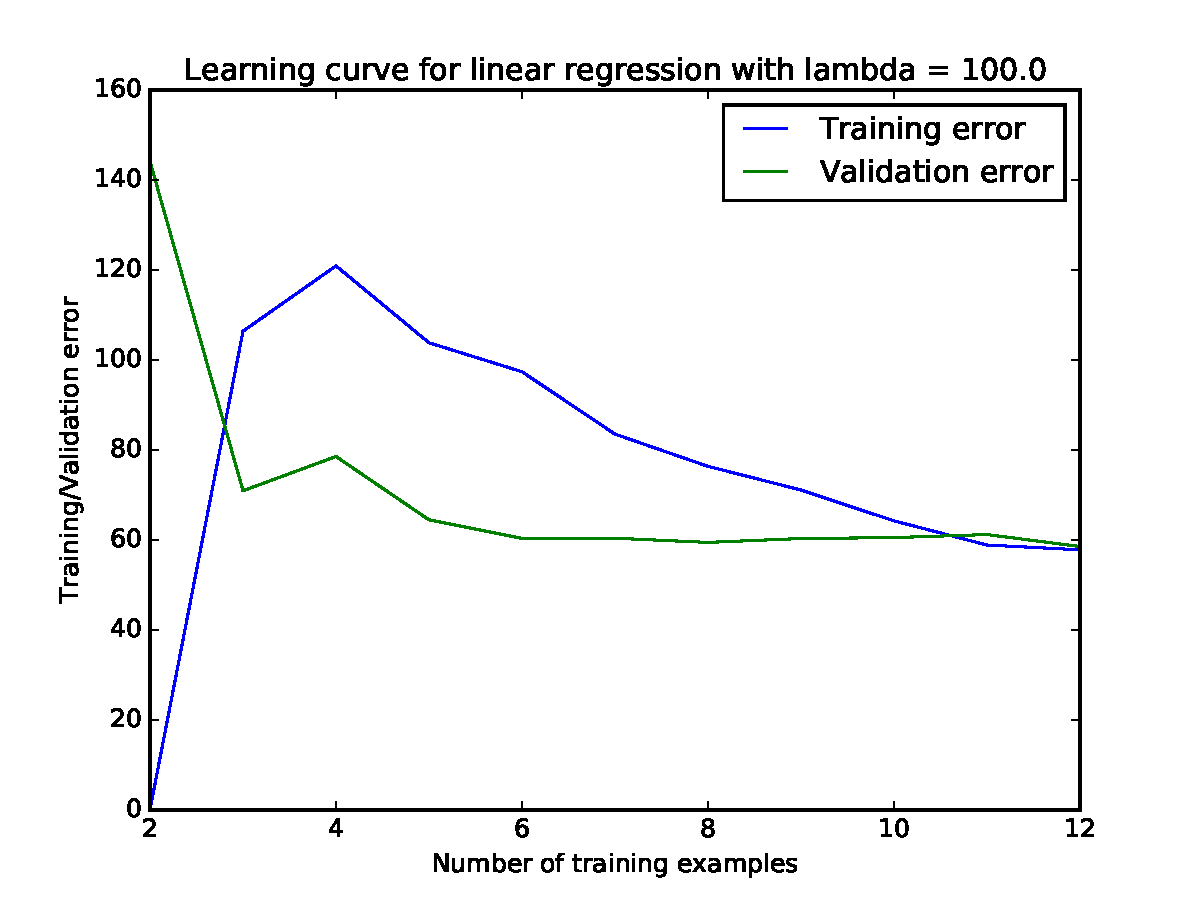
\includegraphics[width=9cm]{part2/fig10_reg100.pdf}}
\caption{Polynomial fits and learning curves for different lambda}\label{fig:9_10_reg}
\end{figure}
\restoregeometry

\subsection{Problem 3.2.A5}
\label{3.2.A5}
\begin{itemize}
\item Completed the \verb|validation_curve| function in the file \verb|utils.py|. The results from \verb|ex2.py| are shown
  in Fig~\ref{fig:12}.
\end{itemize}
Due to randomness in the training and validation splits of the dataset, the cross validation error can sometimes be lower 
than the training error.
We observe that value of $\lambda=1$ is a good choice for the regularization parameter.
\begin{figure}[h]
  \centering{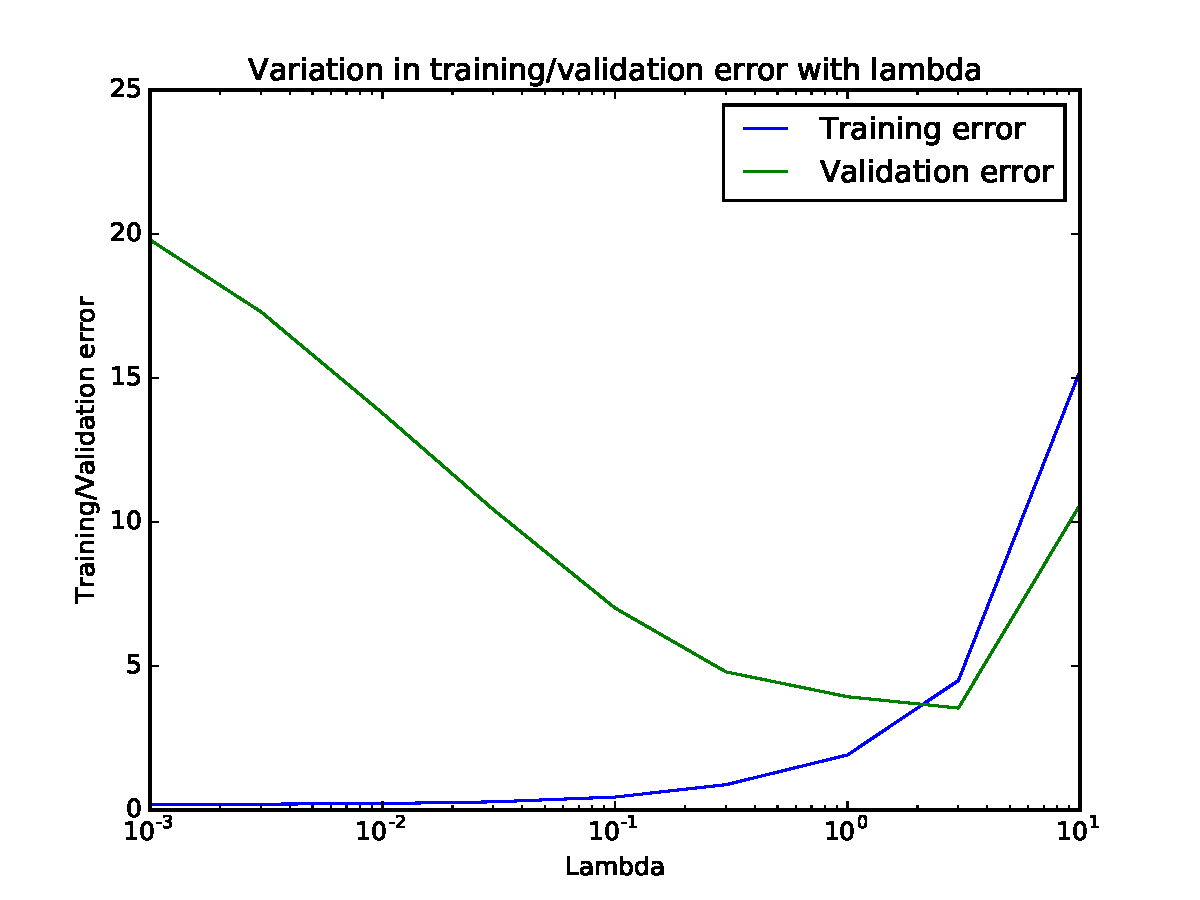
\includegraphics[width=15cm]{part2/fig12.pdf}}
  \caption{Variation in training/validation error with lambda.}\label{fig:12}
\end{figure}

\subsection{Problem 3.2.A6}
\begin{itemize}
\item Per the requirements, added code to \verb|ex2.py|. This uses the best model parameters from section~\ref{3.2.A5} and
  evaluates the error on test data. We picked a value of about $\lambda=1.0$ for the best model.
  The output is
\begin{verbatim}
Theta at lambda = 1.0 (problem3.2.A6) is  [ 11.21759608   8.38067931   5.21899733   3.62613424   2.11030661
   1.95470373   0.78523708]
Error at lambda = 1.0 (problem3.2.A6) is  3.0987791808
\end{verbatim}
\end{itemize}

\subsection{Problem 3.2.A7}
\begin{itemize}
\item Completed the \verb|averaged_learning_curve| function in the file \verb|utils.py| per the requirements of the problem.
\end{itemize}
The output from \verb|ex2.py| is plotted in Fig~\ref{fig:11}
\begin{figure}[h]
  \centering{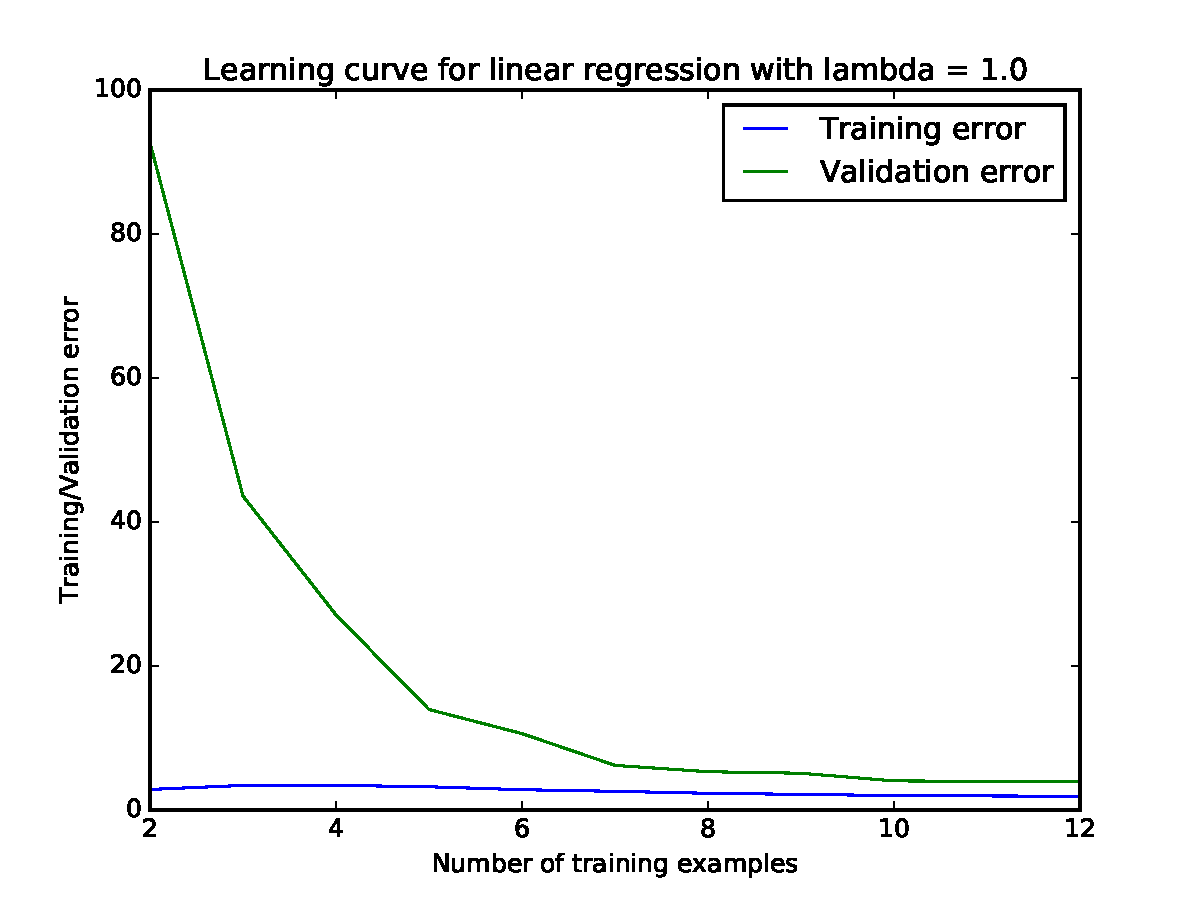
\includegraphics[width=15cm]{part2/fig11.pdf}}
  \caption{Averaged learning curves for lambda=1.}\label{fig:11}
\end{figure}
\end{document}
